\documentclass[preprint,11pt]{elsarticle}
\usepackage[T1]{fontenc}
\usepackage[utf8]{inputenc}
\usepackage{newtxtext,newtxmath}
\usepackage{amsmath,mathtools}
\usepackage{booktabs,array,tabularx,longtable}
\usepackage{graphicx}
\usepackage{microtype}
\usepackage{enumitem}
\usepackage{url}
\usepackage{hyperref}
\usepackage{caption}
\usepackage{float}
\usepackage{siunitx}
\hypersetup{colorlinks=true,allcolors=blue}
\setlength{\emergencystretch}{3em}
\journal{Knowledge-Based Systems}

\begin{document}
\begin{frontmatter}

\title{Differentiable Ultrametric Routing for Hierarchical Evidence under Uncertain Provenance}
\author{K. A. Ulizko, A. S. Vatian, M. V. Ulizko, I. V. Tomilov, N. F. Gusarova}

\begin{abstract}
Knowledge-based systems often combine learned semantic evidence with hierarchical knowledge such as taxonomies, ontologies, or provenance labels. When structural assignments are uncertain, exact-support commitment to one selected branch can create brittle routing errors. We study this robustness--commitment trade-off using nested prefix-ultrametric shells. Dual-Space Attention (DSA) implements the resulting structural compatibility as a pre-softmax attention bias; the same compatibility can also be applied post-encoder. We derive finite-depth continuous extensions for factorized soft hierarchical passports, prove an explicit cross-depth sensitivity gap, and establish a context-dependent foreign-shell leakage bound.

Controlled depth-four experiments show no detectable accuracy difference between normalized hard gating and fixed ultrametric routing under exact provenance, while a development-tuned prefix-ultrametric schedule slightly outperforms the fixed $\rho=0.2$ schedule. Under 30\% provenance noise, soft telescoping routing reduces catastrophic foreign-branch contamination from 0.199 to 0.033 and modestly improves path accuracy over hard MAP. On WOS-46985 with frozen ModernBERT-base representations, oracle parent information favors hard gating. With model-predicted parents, exact-support hard MAP reaches 0.5287 leaf accuracy, whereas MAP plus finite bias reaches 0.5786: a matched gain of about 0.0499 from removing zero-support commitment while retaining MAP provenance. Preserving the full parent posterior raises accuracy only to 0.5794 ($+0.0008$ versus matched MAP finite bias), and this unperturbed accuracy effect is not robust across inferential procedures; the hierarchy-agnostic classifier reaches 0.5793. Posterior preservation has clearer effects on likelihood, branch concentration, and robustness under stronger controlled corruption. WOS is therefore evidence for the finite-bias routing principle under uncertain provenance, not for general multi-depth ultrametric superiority or end-to-end DSA.
\end{abstract}

\begin{keyword}
hierarchical knowledge \sep uncertain provenance \sep evidence routing \sep ultrametric geometry \sep structural attention \sep robustness
\end{keyword}
\end{frontmatter}

\section{Introduction}
Knowledge-based intelligent systems increasingly combine learned semantic evidence with explicit structural knowledge, including taxonomies, ontologies, provenance chains, hierarchical metadata, retrieval sources, and externally supplied branch assignments. These sources need not agree: a semantically salient item can originate outside the branch relevant to the current decision, while the structural assignment itself can be uncertain. Consider a classifier whose parent predictor is uncertain between two taxonomy branches while leaf-level semantic evidence remains strong in both: collapsing the parent distribution to one MAP branch and then hard-masking the other makes the runner-up branch irrecoverable. Here hierarchical provenance acts as structured knowledge that constrains how evidence is allocated, rather than as another feature concatenated to the semantic representation. The design question is therefore not only whether hierarchical knowledge should constrain inference, but how strongly a system should commit to that knowledge when provenance is imperfect.

We distinguish two design choices that are often conflated. The first is support hardness: whether structural routing assigns exactly zero probability outside a selected branch or instead uses a finite compatibility bias. The second is provenance representation: whether an uncertain branch distribution is collapsed to its MAP value or retained during routing. Exact-support gating is attractive when the branch is known exactly because admissibility is enforced without ambiguity. When the branch is estimated, however, zero-support commitment can make a MAP error brittle. Our experiments separate these factors where possible and show that, on WOS, avoiding zero-support commitment accounts for most of the robustness gain, while posterior preservation has a smaller, metric- and corruption-dependent effect. The objective is not universal improvement in semantic classification, but controlled use of structural knowledge under uncertain provenance.

We realize this principle through nested common-prefix shells. For root-to-node addresses, the finite prefix ultrametric
\begin{equation}
 d_\rho(x,y)=\rho^{\operatorname{lcp}(x,y)}\quad(x\neq y),\qquad d_\rho(x,x)=0,\qquad 0<\rho<1
 \label{eq:ultra}
\end{equation}
encodes how deeply two items share a hierarchical prefix. The metric is classical. We do not claim the introduction of hierarchical compatibility, ultrametric attention, or uncertainty-aware routing in isolation. Rather, we formalize their interaction when hierarchical provenance is uncertain: we separate support hardness from posterior representation, construct finite-depth continuous extensions that recover the same hard hierarchy on exact assignments, and characterize how hard-equivalent extensions can differ away from those vertices. Dual-Space Attention (DSA) is an attention-level realization of this routing principle. A $p$-adic address with $\rho=1/p$ is one exact algebraic realization, not a required numerical substrate or a claim of uniquely optimal decay.

The empirical design separates insertion point from routing principle. In controlled synthetic experiments, DSA is evaluated directly as a pre-softmax structural bias inside attention, where true provenance, evidence salience, and branch membership are observable. In the external natural-language experiment, a frozen pretrained encoder supplies document representations and the same hard-versus-soft hierarchical compatibility is applied post-encoder. The external assay therefore tests transfer of uncertainty-aware routing, not end-to-end insertion of DSA into ModernBERT self-attention.

The theory addresses two questions specific to soft provenance. First, we derive finite-depth telescoping and exponential extensions that agree on every hard address, including the zero diagonal, but propagate sensitivity differently across depth. At a symmetric soft point, an operational cross-depth sensitivity ratio exhibits an explicit factor $\rho^{-(D-1)}C(\rho,s,D)$, with $C$ bounded in depth for fixed interior $\rho,s$. Second, we bound foreign-shell attention leakage using the structural logit gap, semantic-logit magnitude, and the number of visible foreign items.

The experiments likewise separate distinct questions about support hardness and provenance representation. A depth-four controlled assay compares vanilla, Euclidean-address, tree-distance, fitted Poincar\'e, shuffled-taxonomy, normalized-hard, fixed-ultrametric, and development-tuned prefix-ultrametric alternatives. Difficulty, provenance-noise, missing-provenance, and salience-shift tests identify the robustness--commitment trade-off. WOS-46985 then tests the same commitment distinction with real text, a released hierarchy, and independently pretrained ModernBERT representations.

We evaluate three separable hypotheses. H1 asks whether exact support is brittle when provenance is uncertain; the matched WOS ablation directly isolates this factor. H2 asks whether retaining the full provenance posterior adds value once support is finite; this is tested by posterior versus matched MAP finite-bias routing. H3 asks whether shared-prefix ultrametric geometry is useful under genuine multi-depth structure; this is evaluated primarily in the controlled depth-four hierarchy rather than inferred from shallow WOS.

The paper makes four contributions. First, it formulates hierarchical provenance as uncertain structural knowledge and distinguishes provenance representation from support hardness. Second, it introduces differentiable finite-depth prefix-based compatibility functions and an attention-level DSA realization that recover the same hard hierarchy on exact assignments while permitting controlled off-branch support. Third, it characterizes the non-uniqueness of continuous extensions of the same hard hierarchy through a depth-sensitivity theorem and derives a context-dependent worst-case leakage bound. Fourth, it empirically isolates the mechanisms: controlled multi-depth experiments test shared-prefix geometry, while the external WOS assay shows that avoiding zero-support commitment is the dominant source of its robustness gain over Hard MAP, rather than preservation of the complete provenance posterior. The resulting claim is conditional: uncertain structural knowledge should not automatically be converted into zero-support commitment; posterior preservation is a separate design choice; and ultrametric shells are one controlled realization rather than a universally superior geometry.

\section{Related Work}
\subsection{Knowledge-guided routing and uncertain structure}
Knowledge-based systems combine learned representations with explicit structure through knowledge-graph augmentation, retrieval, and constrained decoding [1--5]. Neural attention also accepts structural information through relation-dependent biases, graph encodings, structured self-attention, and sparse support constraints [6--13]. DSA belongs to this broad family, but the structural relation is the nested shell induced by hierarchical provenance.

A complementary literature treats uncertainty in structured knowledge as first-class rather than binary. Knowledge Vault estimates fact correctness during fusion [14], uncertain knowledge-graph embeddings retain confidence scores [15], Probabilistic Soft Logic relaxes logical constraints [16], and entity linking naturally maintains multiple structural hypotheses before disambiguation [17]. Our setting is narrower: the uncertain variable is hierarchical provenance, and the operational question is whether its distribution should be collapsed before it modulates evidence routing.

\subsection{Hierarchy geometry and continuous structural variables}
Hyperbolic representations and neural architectures are widely used for tree-like data [18--24]. They motivate a direct comparison rather than an assumption of inferiority; our controlled assay therefore includes a 10-dimensional Poincar\'e embedding fitted to the same taxonomy under a matched development-tuning budget. Prefix or Baire ultrametrics encode hierarchy through longest common prefix [25], while classical work establishes finite Euclidean realizations and related kernel facts [26--28]. Recent non-Archimedean machine learning includes $p$-adic learning primitives, ultrametric representation learning, broader non-Archimedean formulations, adelic embeddings, and a deterministic ultrametric-attention proof of concept [29--34].

The closest attention-specific antecedent is Quni-Gudzinas [34], which uses a binary-tree proxy encoder and an ultrametric LCA matrix in a small deterministic synthetic demonstration. We do not claim novelty for ultrametric attention itself. The present work changes the question to routing under uncertain hierarchical provenance: addresses may be exact, missing, or probabilistic; the construction is finite-depth and differentiable; the analysis covers hard-vertex exactness, soft-address depth sensitivity, and foreign-shell leakage; and the empirical program combines depth-four interventions with WOS-46985 transfer.

Continuous relaxations such as Gumbel-softmax and Concrete distributions [35,36] and alternative probability mappings such as sparsemax and entmax [37,38] provide general machinery for uncertain categorical variables. Our per-level simplex representation is standard; the substantive issue is its composition through a prefix scan, because continuous extensions that agree at every discrete address can have very different cross-depth sensitivity away from those vertices. Hierarchical text classification [39,40] supplies an external setting in which semantic class evidence and parent-branch information can be observed separately. We use ModernBERT [41] only as a frozen representation source, so the WOS experiment evaluates post-encoder routing rather than an end-to-end modification of its internal attention.

\section{Problem Formulation: Hierarchical Knowledge under Uncertain Provenance}
Let $\mathcal O$ be a rooted hierarchy and let semantic evidence for a query or instance induce logits $E_j$ over candidate items or output concepts $j$. Independently, structural information induces a hierarchical provenance variable. Under exact provenance this variable is a node or path; under uncertain provenance it is represented by a distribution $q$. In the multi-depth DSA construction, $q$ is represented by level-wise categorical marginals; in WOS it is the complete seven-way parent posterior.

We distinguish three operators. A hierarchy-agnostic decision uses only $E_j$. A hard structural commitment replaces $q$ by its MAP address and gates or strongly suppresses candidates outside that branch. An uncertainty-preserving structural route computes a compatibility $H_j(q,\mathcal O)$ and combines it with semantic evidence before normalization:
\begin{equation}
 \pi(j\mid E,q,\mathcal O)=\operatorname{softmax}_j\bigl(E_j+H_j(q,\mathcal O)\bigr).
 \label{eq:routing}
\end{equation}
The methodological distinction is whether uncertainty is collapsed before structural aggregation.

Equation~\eqref{eq:routing} is insertion-point agnostic. In DSA, $E_{ij}=Q_iK_j^\top/\sqrt{d_k}$ and $H_{ij}$ is a nested-shell pre-softmax bias between query and key passports. In WOS, $E_j$ is a semantic leaf logit from a frozen-encoder head and $H_j$ is a parent-compatibility bias derived from a predicted provenance posterior. The hypothesis is conditional rather than monotone: when provenance is externally known to be exact, hard constraints should be competitive or preferable; when provenance is predicted, finite-bias routing may be more robust than exact-support MAP commitment.

The WOS assay further isolates provenance representation from support hardness through a matched MAP-plus-finite-bias condition: $q$ is replaced by $\delta_{\arg\max q}$ while the same finite ultrametric kernel and validation-selected parameters are retained. This directly measures the incremental effect of preserving the parent posterior under the same finite-bias operator. The synthetic uncertainty assay compares the practically salient endpoints and therefore does not provide the same factorial separation at attention level.

\section{Nested-Shell Ultrametric Realization}
\subsection{Addresses, distance, and kernel interpretation}
Let $\mathcal O$ be a rooted tree of maximum depth $D$. Each outgoing edge receives a distinct nonzero symbol, while 0 is reserved for padding after a concept terminates. A concept $c$ is represented by $a(c)=(a_0(c),\ldots,a_{D-1}(c))$, and $\operatorname{lcp}(c,c')$ is the number of initial coordinates on which two addresses agree. Equation~\eqref{eq:ultra} defines an ultrametric because
\[
\operatorname{lcp}(x,y)\geq \min\{\operatorname{lcp}(x,z),\operatorname{lcp}(z,y)\},
\]
and $\rho^k$ decreases with $k$. If symbols are interpreted as base-$p$ digits and $\rho=1/p$, then for distinct concepts $d_\rho(c,c')=p^{-v_p(a(c)-a(c'))}$, giving an exact $p$-adic realization of common-prefix depth.

For $k=0,\ldots,D-1$, let $B_k[c,c']=\mathbf 1\{\operatorname{lcp}(c,c')\geq k\}$ and $B_D=I$. Each $B_k$ is positive semidefinite after a common permutation into all-ones blocks. Hence, for any non-increasing $f:[0,\infty)\to[0,\infty)$, the radial kernel $K_{cc'}=f(d_\rho(c,c'))$ is positive semidefinite; if $f$ is strictly decreasing on the finite distance set, $K$ is positive definite. In particular, $\exp(-\gamma d_\rho)$ is positive semidefinite for $\gamma\geq0$. This is a classical kernel fact used only to justify the structural-kernel interpretation; proof details and approximate-ultrametric diagnostics are given in the Supplementary Material.

\section{Differentiable Nested-Shell Routing}
\subsection{Soft hierarchical passports}
Let $h_i\in\mathbb R^d$ be a token hidden state. A passport is a stack of categorical distributions
\begin{equation}
 A_i[d]\in\Delta^{q-1},\qquad d=0,\ldots,D-1,
\end{equation}
obtained by lookup or a learned projector. A conceptness gate $g_i\in[0,1]$ indicates whether the token participates in the ontology prior, and a query-side branch-activation gate $r_i\in\{0,1\}$ is zero at the root and one after a non-root hypothesis has been established. Per-level agreement and prefix survival are
\begin{equation}
 S_{ij}[d]=\langle A_i[d],A_j[d]\rangle,\qquad P_{ij}[d]=\prod_{m=0}^{d}S_{ij}[m].
 \label{eq:survival}
\end{equation}
For one-hot passports, $P[d]$ is one until the first mismatch and zero thereafter. The factorized representation preserves the available categorical uncertainty at each level but does not encode arbitrary dependencies among complete paths.

\subsection{Finite-depth continuous extensions}
A finite tree has a true zero diagonal, so a truncated prefix series must explicitly handle the all-match state. With $P[-1]=1$, define the telescoping relaxation
\begin{equation}
 \widetilde d_{\rm tel}=\sum_{k=0}^{D-1}\rho^k\bigl(P[k-1]-P[k]\bigr),
 \label{eq:tel}
\end{equation}
and, with $\widetilde v=\sum_{d=0}^{D-1}P[d]$, the exponential relaxation
\begin{equation}
 \widetilde d_{\rm exp}=\rho^{\widetilde v}-\rho^D P[D-1].
 \label{eq:exp}
\end{equation}
If both passports are one-hot, then
\begin{equation}
 \widetilde d_{\rm tel}(i,j)=\widetilde d_{\rm exp}(i,j)=d_\rho(c_i,c_j)
 \label{eq:hardexact}
\end{equation}
for all pairs, including identical concepts. We call two relaxations hard-equivalent when they coincide with the same finite hard hierarchy for every pair of one-hot passports. Thus the two extensions are hard-equivalent but can differ away from those vertices.

\subsection{Depth-sensitivity theorem}
For a gradient profile $G(m)>0$, define the operational cross-depth sensitivity ratio
\begin{equation}
 \kappa_G(D)=\frac{\max_{0\leq m<D}G(m)}{\min_{0\leq m<D}G(m)}.
 \label{eq:kappa}
\end{equation}
This is a descriptive ratio of gradient magnitudes across hierarchy levels, not the condition number of a Jacobian or Hessian.

\textbf{Theorem 1 (depth-sensitivity gap).} Fix $D\geq2$ and $\rho,s\in(0,1)$ and evaluate at $S[0]=\cdots=S[D-1]=s$. Let $v_D=s(1-s^D)/(1-s)$ and $a_D=(-\ln\rho)\rho^{v_D}$. The derivative magnitudes of Eqs.~\eqref{eq:tel}--\eqref{eq:exp} are
\begin{align}
 G_{\rm tel}(m)&=(1-\rho)\sum_{d=m}^{D-2}(\rho s)^d+(\rho s)^{D-1},\\
 G_{\rm exp}(m)&=a_D\sum_{d=m}^{D-1}s^d+\rho^D s^{D-1}.
\end{align}
Both profiles are strictly decreasing in $m$, and
\begin{equation}
 \frac{\kappa_{\rm tel}(D)}{\kappa_{\rm exp}(D)}=\rho^{-(D-1)}C(\rho,s,D),
 \label{eq:gap}
\end{equation}
where for every fixed interior $\rho,s$ there exist positive finite constants $c_1(\rho,s),c_2(\rho,s)$, independent of $D$, such that $c_1\leq C(\rho,s,D)\leq c_2$. For the $p$-adic specialization $\rho=1/p$, the explicit leading factor is $p^{D-1}$.

The proof follows by differentiating prefix survival, establishing strict monotonicity through consecutive differences, and uniformly bounding the residual factor $C$; explicit constants and the complete derivation are provided in the Supplementary Material. An executable verification over 3,888 $(\rho,s,D)$ grid points found no monotonicity or bound violation and a worst relative identity error of $1.1\times10^{-14}$.

Practically, Theorem 1 establishes non-uniqueness of a soft relaxation: hard-equivalent functions can encode identical exact hierarchical decisions yet propagate uncertainty across depth differently. It is a local sensitivity result for the passport-composition operator, not a claim of globally better conditioning or easier optimization. Once exact constraints are relaxed, the continuous extension is therefore a substantive modeling choice rather than an implementation detail.

\begin{figure}[H]
\centering
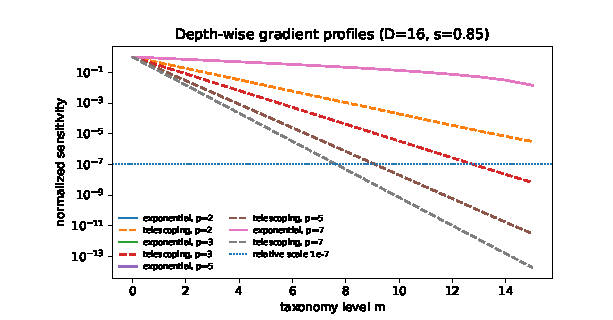
\includegraphics[width=.55\linewidth]{figures/fig_gradients.pdf}
\caption{Finite-depth gradient profiles. The telescoping extension carries additional geometric attenuation across depth.}
\label{fig:grad}
\end{figure}

\subsection{Attention-level DSA, strictness, and leakage}
A direct penalty $-\gamma g_i g_j\widetilde d$ makes a nonconcept token relatively attractive whenever $g_j=0$. We therefore use the similarity form
\begin{equation}
 B_{ij}=\gamma r_i g_i g_j\bigl(1-\widetilde d(i,j)\bigr),\qquad
 A=\operatorname{softmax}\left(\frac{QK^\top}{\sqrt{d_k}}+B+C\right).
 \label{eq:dsa}
\end{equation}
For an active non-root query with ontological visible tokens, this is softmax-equivalent to the penalty form up to a query-wise constant. Nonconcept tokens remain neutral, and $r_i=0$ at the root prevents padding or unknown mass from manufacturing a structural preference before a branch exists.

For hard concept pairs with common-prefix depths $k$ and $k+1$, the adjacent-shell structural logit gap is
\begin{equation}
 \Delta_k=\gamma(1-\rho)\rho^k,
\end{equation}
so maintaining separation at least $\tau$ through depth $k$ requires $\gamma\geq\tau/[(1-\rho)\rho^k]$. Small $\rho$ strengthens coarse separation but compresses deep-shell gaps.

A complementary leakage result relates structural separation to semantic competition. Let $z_{ij}=E_{ij}+H_{ij}$, let $B\subseteq V_i$ be a nonempty nearest shell with structural logit $H_i^*$, assume $|E_{ij}|\leq E_{\max}$, and define
\[
\Delta_i=\min_{j\in V_i\setminus B}(H_i^*-H_{ij})>0.
\]
Then
\begin{equation}
 \sum_{j\in V_i\setminus B}A_{ij}
 \leq \min\left\{1,\;|V_i\setminus B|\exp(2E_{\max}-\Delta_i)\right\},
 \label{eq:leak}
\end{equation}
and a sufficient condition for leakage at most $\varepsilon$ is $\Delta_i\geq2E_{\max}+\log(|V_i\setminus B|/\varepsilon)$. Equation~\eqref{eq:leak} is a worst-case sufficient bound under the stated assumptions, not an empirically calibrated predictor of observed leakage. The cardinality term is essential: exponential suppression in the structural gap does not imply context-length invariance. Agreement computation costs $O(L^2Dq)$, the prefix scan $O(L^2D)$, and a materialized mask $O(L^2)$ memory. Full proofs are deferred to the Supplementary Material.

\section{Controlled Mechanism Validation}
\subsection{Protocol and baselines}
The synthetic generator is designed for attention-level mechanism identification: true taxonomy, evidence provenance, and salience are observable, allowing one structural factor to vary while the rest are held fixed. The canonical hierarchy has depth four and branching factor three. Full-path accuracy requires every teacher-forced child decision to be correct. DSA is applied directly inside attention. Exact-provenance comparisons use ten held-out seeds with 300 traces per seed; corruption comparisons use ten held-out seeds with 800 traces per seed. Hyperparameters are selected on development seed 0 and then fixed; no test-set tuning is used. We report mean$\pm$SD and, for superiority claims, paired mean differences, 95\% $t$ intervals, Cohen's $d_z$, and exact paired sign-flip tests. To keep inference focused, the reporting hierarchy designates four primary contrasts: hard routing versus fixed ultrametric routing in the controlled hierarchy; fixed versus tuned prefix-ultrametric routing; WOS Hard MAP versus matched MAP plus finite bias; and WOS matched MAP finite bias versus posterior finite bias. Other comparisons are secondary or exploratory.

Baselines are vanilla attention, Euclidean padded-address similarity, ordinary tree-distance similarity, a taxonomy-fitted 10-dimensional Poincar\'e similarity, shuffled taxonomy, a filler-normalized hard gate, fixed ultrametric routing, and a development-tuned prefix-ultrametric control. Poincar\'e coordinates are fitted only to taxonomy similarity (mean absolute similarity error 0.0036). The dimension is fixed at 10 before test evaluation and serves as a fixed hyperbolic comparator; structural-scale tuning uses the same development protocol as for competing structural baselines. The tuned prefix-ultrametric control selects decay base 0.33 rather than the fixed 0.2 schedule, with the zero diagonal unchanged; it tests whether that fixed schedule is privileged within the same family.

For uncertain provenance, hard MAP collapses each observed level distribution to one symbol, whereas soft exponential and telescoping routing consume the full available per-level passport distributions. Catastrophic foreign-branch contamination is the fraction of traces in which any non-root decision assigns more than 50\% of attention mass to truly foreign concepts.

\subsection{Exact provenance and difficulty continuum}
Table~\ref{tab:exact} reports the canonical exact-provenance audit. Fixed ultrametric routing reaches $0.6173\pm0.0176$, above ordinary tree distance and the fitted Poincar\'e baseline. The paired ultrametric--Poincar\'e difference is $+0.1493$ (95\% CI $[0.1343,0.1644]$, $d_z=7.11$, exact sign-flip $p=0.00195$). Shuffling the taxonomy while retaining the same structural-bias machinery reduces accuracy to $0.0133\pm0.0087$; this negative control indicates that the gain depends on meaningful hierarchy rather than on an arbitrary extra bias term. Two controls further delimit the claim: normalized hard gating reaches $0.6183\pm0.0224$ with no detectable difference from fixed ultrametric routing, whereas the tuned prefix-ultrametric schedule reaches $0.6230\pm0.0192$ and exceeds the fixed $\rho=0.2$ schedule by $0.0057$ (95\% CI $[0.0010,0.0103]$, $p=0.0156$). The controlled experiment therefore supports usefulness of shared-prefix ultrametric structure for this tested multi-depth routing problem, not general superiority of ultrametrics for hierarchical learning.

\begin{table}[H]
\centering
\caption{Exact-provenance audit, ten held-out seeds (300 traces per seed).}
\label{tab:exact}
\begin{tabular}{lr}
\toprule
Method & Full-path accuracy\\
\midrule
Vanilla & $0.0007\pm0.0014$\\
Euclidean address & $0.0287\pm0.0077$\\
Tree distance & $0.1497\pm0.0235$\\
Fitted Poincar\'e (10D) & $0.4680\pm0.0278$\\
Shuffled taxonomy & $0.0133\pm0.0087$\\
Fixed ultrametric ($\rho=.2$) & $0.6173\pm0.0176$\\
Tuned prefix-ultrametric ($a=.33$) & $0.6230\pm0.0192$\\
Hard gate + filler normalization & $0.6183\pm0.0224$\\
\bottomrule
\end{tabular}
\end{table}

The effect is not restricted to one adversarial operating point. Increasing foreign-evidence pressure continuously from an easy regime ($\lambda=0$) to the canonical regime ($\lambda=1$) degrades vanilla from 0.317 to approximately zero and tree distance from 0.508 to 0.140, whereas ultrametric routing remains at 0.607 and normalized hard routing follows the same high-performing regime. The detailed curve is shown in Fig.~\ref{fig:difficulty}; the redundant exact-provenance summary figure is moved to the Supplementary Material.

\begin{figure}[H]
\centering
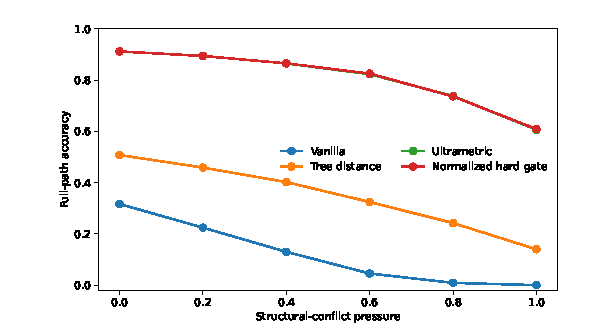
\includegraphics[width=.58\linewidth]{figures/fig_difficulty_continuum.pdf}
\caption{Difficulty continuum (five seeds). Structural-conflict pressure increases continuously from an easy regime to the canonical adversarial regime.}
\label{fig:difficulty}
\end{figure}

\subsection{Uncertain provenance and salience shift}
Direct passport optimization agrees with the theorem's practical direction: both relaxations recover all prefixes through depth eight; at depth 12 the telescoping form reaches 10 levels at the 90\% criterion while the exponential form reaches 12, and at depths 16--96 they plateau near 10 and 14 levels, respectively. Full optimization diagnostics are reported in the Supplementary Material because they concern learning soft passports rather than consuming already uncertain passports.

Table~\ref{tab:uncertain} gives the central uncertainty audit. Under 30\% noisy provenance, soft telescoping improves path accuracy over hard MAP by $+0.0161$ (95\% CI $[0.0067,0.0255]$, $d_z=1.23$, $p=0.00391$) and reduces catastrophic contamination by $-0.1658$ (95\% CI $[-0.1759,-0.1556]$, $p=0.00195$). Soft exponential has the same qualitative pattern. Under 35\% missing provenance, hard MAP remains more accurate, but both soft rules approximately halve catastrophic contamination. Because MAP collapse and exact-support gating change together in this synthetic comparison, the result establishes robustness of the composite soft finite-bias operator rather than attributing the entire effect uniquely to posterior preservation.

\begin{table}[H]
\centering
\caption{Uncertain-provenance audit, ten held-out seeds (800 traces per seed). Cat. = catastrophic foreign-branch contamination rate.}
\label{tab:uncertain}
\begin{tabular}{llcc}
\toprule
Regime & Method & Path accuracy & Cat.\\
\midrule
Noisy 30\% & Hard MAP & $0.0995\pm0.0071$ & $0.1988\pm0.0165$\\
& Soft exponential & $0.1118\pm0.0154$ & $0.0606\pm0.0072$\\
& Soft telescoping & $0.1156\pm0.0152$ & $0.0330\pm0.0045$\\
\addlinespace
Missing 35\% & Hard MAP & $0.1131\pm0.0090$ & $0.1383\pm0.0087$\\
& Soft exponential & $0.0839\pm0.0099$ & $0.0670\pm0.0080$\\
& Soft telescoping & $0.0914\pm0.0109$ & $0.0763\pm0.0099$\\
\bottomrule
\end{tabular}
\end{table}

An out-of-distribution salience sweep gives the operational consequence of this difference. At 30\% noisy provenance, raising foreign-evidence loudness from 0 to 2.5 increases hard-MAP catastrophic contamination from 0.092 to 0.299, while soft telescoping rises only from 0.033 to 0.057; path accuracy remains approximately 0.118 to 0.115 for soft telescoping but falls from 0.120 to 0.098 for hard MAP. Figure~\ref{fig:salience} summarizes the robustness curve. A paired wrong-vote-location intervention and a secondary pretrained-synthetic compatibility control are retained in the Supplementary Material; together they show that routing responds to evidence provenance rather than logical polarity and that the structural ranking does not depend on an ontology-specific pretrained encoder.

\begin{figure}[H]
\centering
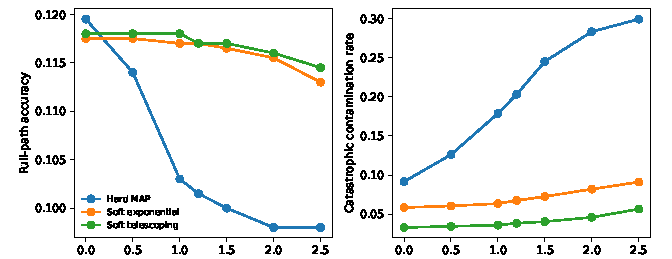
\includegraphics[width=.72\linewidth]{figures/fig_uncertain_provenance.pdf}
\caption{Operational robustness under foreign-salience shift. Soft routing stabilizes both path accuracy and catastrophic foreign-branch contamination under noisy provenance.}
\label{fig:salience}
\end{figure}

\section{External Transfer on Real Hierarchical Text Data}
\subsection{Protocol and scope}
WOS-46985 contains 46,985 scientific abstracts, 134 released flat target classes, and seven top-level domains [39,40]. This external assay is explicitly post-encoder: it validates the hierarchical routing principle on frozen natural-language representations, not the complete attention-level DSA architecture. We use one fixed 70/15/15 split stratified by the 134-way target, yielding 32,889 training, 7,048 validation, and 7,048 test documents. The public hierarchy metadata contain sparse inconsistencies: three released flat identifiers occur with more than one observed top-level label and only 133 distinct $(YL1,YL2)$ pairs occur. We retain the released 134-way $Y$ field as the leaf target and derive a deterministic 134-to-7 leaf--parent map from training rows only, assigning each leaf to its modal training $YL1$ parent. Mean training parent purity is 0.9974 (minimum 0.7731); validation and test labels never determine this map.

We use answerdotai/ModernBERT-base [41] as a frozen external encoder. Abstracts are truncated to 512 tokens, encoded once, and mean-pooled over non-padding last-layer representations. For each of ten paired random seeds, two linear heads are trained on the same frozen representation: a seven-way parent head and a hierarchy-agnostic 134-way semantic leaf head. Separate scalar temperatures are fitted on validation NLL. The parent head reaches $0.7677\pm0.0021$ test accuracy and the semantic leaf head $0.5793\pm0.0020$.

Let $E_c=z_c^{\rm leaf}/T_{\rm leaf}$, $s_c=\operatorname{softmax}_c(E)$, $q_b=\operatorname{softmax}_b(z^{\rm parent}/T_{\rm parent})$, and let $g(c)$ map leaf $c$ to its train-derived parent. For each finite-bias method $m$, let $K^{(m)}_{bc}>0$ be the parent-to-leaf compatibility computed from the train-derived hierarchy. Distributional finite-bias routing is
\begin{equation}
 C_c^{(m)}(q)=\sum_{b=1}^{7}q_bK^{(m)}_{bc},\qquad
 \pi_c^{(m)}=\frac{s_cC_c^{(m)}(q)}{\sum_k s_kC_k^{(m)}(q)}.
 \label{eq:wossoft}
\end{equation}
Hard MAP instead sets $\widehat b=\arg\max_b q_b$ and
\begin{equation}
 \pi_c^{\rm hard}=\frac{s_c\mathbf 1\{g(c)=\widehat b\}}{\sum_{k:g(k)=\widehat b}s_k},
 \label{eq:woshard}
\end{equation}
so leaves outside the selected branch receive exactly zero routed probability. Throughout, zero support means that the structural routing operator makes candidates outside the selected branch inadmissible before normalization; it is distinct from a finite-support softmax weight that may become numerically small after normalization. The matched MAP-plus-finite-bias control uses $q_{\rm MAP}=\delta_{\widehat b}$ in Eq.~\eqref{eq:wossoft} while retaining exactly the same ultrametric kernel and validation-selected parameters as posterior finite-bias routing. All routing parameters are selected using validation data and frozen before test evaluation; no test-set tuning or retuning is performed for the matched control.

For reporting NLL only, true-class probability is clipped below at $10^{-12}$; this floor is not applied to predictions, ECE, or hierarchical-risk metrics. We report leaf accuracy, macro-F1, NLL, ECE, wrong-parent rate, mean wrong-branch posterior mass, and whether aggregate mass outside the gold parent exceeds 0.5. Because WOS has only one meaningful parent-to-leaf transition, leaf and path accuracy coincide. Replication across ten head seeds estimates run-to-run variability from fitted heads and initialization, whereas the document bootstrap quantifies evaluation-sample uncertainty conditional on the fixed split and fitted seed ensemble. For three interpretation-critical contrasts, per-document differences are averaged across seeds and 20,000 resamples of the 7,048 fixed test documents produce percentile 95\% intervals.

\subsection{Oracle versus predicted provenance}
With oracle gold-parent input, hard gating reaches $0.6855\pm0.0027$ leaf accuracy while finite-bias ultrametric routing reaches $0.6029\pm0.0019$; the paired ultrametric--hard difference is $-0.0826$ (95\% CI $[-0.0843,-0.0809]$, exact sign-flip $p=0.00195$). Because the posterior is one-hot, matched MAP-plus-finite-bias and posterior finite-bias routing coincide. Exact branch knowledge therefore favors exact-support commitment in this assay.

With model-predicted parents, the primary external contrast is Hard MAP versus matched MAP plus finite bias: accuracy rises from $0.5287\pm0.0020$ to $0.5786\pm0.0015$, a gain of about 0.0499 obtained by removing zero-support commitment while keeping MAP provenance. Posterior finite-bias ultrametric routing reaches $0.5794\pm0.0016$ and vanilla $0.5793\pm0.0020$. Thus the matched control recovers almost the entire hard-versus-posterior gap before posterior preservation is introduced. Table~\ref{tab:wos} reports the full comparison.

\begin{table}[H]
\centering
\caption{WOS-46985 with model-predicted branch assignments, ten paired head seeds. Lower is better for NLL, ECE, and hierarchical-risk metrics.}
\label{tab:wos}
\scriptsize
\begin{tabular}{lcccc}
\toprule
\multicolumn{5}{l}{\textit{Panel A: classification and calibration}}\\
Method & Accuracy & Macro-F1 & NLL & ECE\\
\midrule
Vanilla & $.5793\pm.0020$ & $.5737\pm.0021$ & $1.5791\pm.0024$ & $.0335\pm.0035$\\
Hard MAP & $.5287\pm.0020$ & $.5216\pm.0034$ & $7.2086\pm.0598$ & $.1272\pm.0016$\\
MAP + finite bias & $.5786\pm.0015$ & $.5725\pm.0021$ & $1.5813\pm.0032$ & $.0349\pm.0020$\\
Tree kernel & $.5796\pm.0016$ & $.5734\pm.0023$ & $1.5773\pm.0029$ & $.0342\pm.0014$\\
Poincar\'e (10D) & $.5797\pm.0017$ & $.5736\pm.0021$ & $1.5772\pm.0026$ & $.0337\pm.0018$\\
Ultrametric & $.5794\pm.0016$ & $.5733\pm.0022$ & $1.5770\pm.0028$ & $.0337\pm.0019$\\
Tuned prefix-ultrametric & $.5794\pm.0017$ & $.5732\pm.0023$ & $1.5769\pm.0027$ & $.0338\pm.0025$\\
\midrule
\multicolumn{5}{l}{\textit{Panel B: hierarchical risk}}\\
Method & Wrong-parent & Wrong-branch mass & Outside-gold $>.5$ & \\
\midrule
Vanilla & $.2005\pm.0027$ & $.2775\pm.0012$ & $.2300\pm.0021$ & \\
Hard MAP & $.2323\pm.0021$ & $.2323\pm.0021$ & $.2323\pm.0021$ & \\
MAP + finite bias & $.1937\pm.0015$ & $.2590\pm.0009$ & $.2179\pm.0016$ & \\
Tree kernel & $.1943\pm.0016$ & $.2613\pm.0009$ & $.2196\pm.0019$ & \\
Poincar\'e (10D) & $.1952\pm.0018$ & $.2639\pm.0019$ & $.2212\pm.0021$ & \\
Ultrametric & $.1953\pm.0022$ & $.2638\pm.0009$ & $.2210\pm.0018$ & \\
Tuned prefix-ultrametric & $.1954\pm.0021$ & $.2638\pm.0012$ & $.2209\pm.0016$ & \\
\bottomrule
\end{tabular}
\end{table}

Preserving the full parent posterior has a much smaller, metric-dependent effect once the finite-bias kernel is fixed. Relative to matched MAP-plus-finite-bias routing, posterior routing changes accuracy by $+0.000851$: the exact paired sign-flip test gives $p=0.0391$, whereas the paired $t$ interval $[-0.000005,0.001707]$ includes zero. Posterior routing reduces NLL by $-0.004369$ (95\% CI $[-0.004802,-0.003936]$, $p=0.00195$). It also increases wrong-parent rate, wrong-branch mass, and the outside-gold-parent $>0.5$ rate in the unperturbed predicted condition, consistent with leaving probability on plausible alternative branches. Table~\ref{tab:matched} reports this matched ablation.

\begin{table}[H]
\centering
\caption{Matched provenance-representation ablation under model-predicted WOS parents. $\Delta$ is posterior finite-bias minus matched MAP finite-bias.}
\label{tab:matched}
\scriptsize
\begin{tabular}{lcccc}
\toprule
Metric & Posterior + finite bias & MAP + finite bias & $\Delta$ & 95\% CI\\
\midrule
Leaf accuracy & $.5794\pm.0015$ & $.5786\pm.0015$ & $+.000851$ & $[-.000005,.001707]$\\
NLL & $1.5770\pm.0028$ & $1.5813\pm.0032$ & $-.004369$ & $[-.004802,-.003936]$\\
Wrong-parent & $.1953\pm.0021$ & $.1937\pm.0015$ & $+.001603$ & $[.000326,.002881]$\\
Wrong-branch mass & $.2638\pm.0009$ & $.2590\pm.0009$ & $+.004744$ & $[.004562,.004925]$\\
Outside-gold $>.5$ & $.2210\pm.0018$ & $.2179\pm.0016$ & $+.003051$ & $[.001601,.004500]$\\
\bottomrule
\end{tabular}
\end{table}

The document bootstrap leads to the same substantive interpretation (Table~\ref{tab:boot}). MAP plus finite bias exceeds exact-support hard MAP by $+0.04987$ accuracy (95\% bootstrap CI $[0.04425,0.05565]$). In contrast, posterior preservation adds $+0.00084$ accuracy relative to matched MAP finite bias, with a bootstrap interval crossing zero, while NLL improves by $-0.00437$. Relative to vanilla, posterior finite-bias routing again shows no detectable accuracy difference. The very large NLL contrast between MAP finite bias and exact-support hard MAP is dominated by zero-probability branch errors evaluated under the stated $10^{-12}$ reporting floor; it should not be interpreted as an ordinary calibration gain of comparable magnitude.

\begin{table}[H]
\centering
\caption{Paired document-bootstrap sensitivity analysis for key WOS contrasts. Differences are first method minus second method; percentile 95\% CIs use 20,000 resamples of 7,048 fixed test documents.}
\label{tab:boot}
\scriptsize
\setlength{\tabcolsep}{3.5pt}
\resizebox{\linewidth}{!}{%
\begin{tabular}{lccc}
\toprule
Contrast & Accuracy $\Delta$ [95\% CI] & NLL $\Delta$ [95\% CI] & OutsideGold50 $\Delta$ [95\% CI]\\
\midrule
MAP+FB $-$ Hard MAP & $+.04987$ $[.04425,.05565]$ & $-5.62723$ $[-5.86099,-5.39603]$ & $-.01436$ $[-.02033,-.00850]$\\
Posterior $-$ MAP+FB & $+.00084$ $[-.00024,.00190]$ & $-.00437$ $[-.00590,-.00284]$ & $+.00308$ $[.00121,.00495]$\\
Posterior $-$ Vanilla & $+.00007$ $[-.00104,.00114]$ & $-.00213$ $[-.00407,-.00018]$ & $-.00897$ $[-.01061,-.00734]$\\
\bottomrule
\end{tabular}%
}
\end{table}

The paired sign-flip test detects a small accuracy difference, whereas both the paired $t$ interval and document-bootstrap interval include zero. Given the effect size ($+0.00085$) and its sensitivity to inferential procedure, we do not treat unperturbed leaf accuracy as a robust benefit of posterior preservation. Clearer effects appear in NLL, branch concentration, and robustness under stronger controlled corruption.

The four distributional soft kernels remain numerically similar on WOS because the released taxonomy contains only one meaningful parent-to-leaf transition; after tuning, tree, Poincar\'e, fixed-ultrametric, and tuned prefix-ultrametric compatibilities are largely alternative parameterizations of within-parent versus cross-parent preference. WOS therefore cannot independently test multi-depth longest-common-prefix geometry. The depth-four synthetic assay identifies that geometry; WOS tests finite-bias hierarchical routing under uncertain provenance on real text and a pretrained representation model. Additional paired risk-difference statistics are moved to the Supplementary Material.

\subsection{Controlled corruption stress test}
We perturb each predicted parent posterior as
\begin{equation}
 q^{(\varepsilon)}=(1-\varepsilon)q+\varepsilon r,
\end{equation}
where $r$ is a one-hot distribution on one randomly selected non-gold parent held fixed for that document and seed, and $\varepsilon\in\{0,0.1,0.2,0.3,0.4\}$. This is a mechanistic stress test, not a model of real-world corruption prevalence.

At $\varepsilon=0.3$, posterior finite-bias ultrametric routing reaches $0.5783\pm0.0021$ accuracy, matched MAP finite bias $0.5767\pm0.0013$, and exact-support hard MAP $0.4951\pm0.0026$. At $\varepsilon=0.4$, hard MAP falls to $0.4022\pm0.0031$, while matched MAP finite bias remains at $0.5758\pm0.0017$ and posterior finite bias at $0.5777\pm0.0019$. Relative to the matched MAP control at this strongest perturbation, preserving the posterior improves accuracy by $+0.00189$ (95\% CI $[0.00116,0.00262]$), lowers the outside-gold-parent $>0.5$ rate by $-0.00613$ (95\% CI $[-0.00710,-0.00516]$), and lowers NLL by $-0.00893$ (95\% CI $[-0.00920,-0.00865]$). Thus finite-bias routing accounts for the dominant robustness gain in this external assay, while posterior preservation can provide a smaller additional benefit under stronger corruption.

\begin{figure}[H]
\centering
\begin{minipage}[t]{0.48\linewidth}
\centering
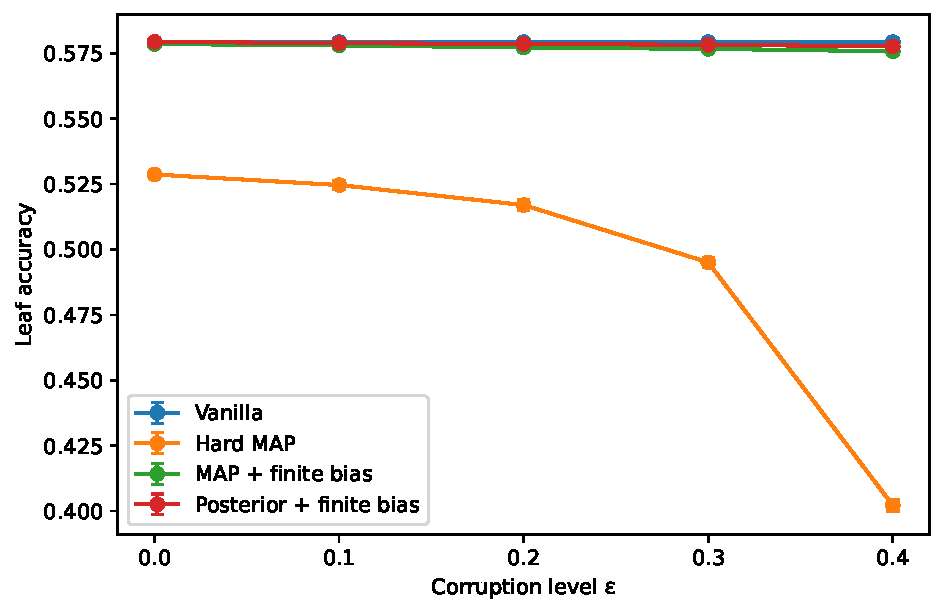
\includegraphics[width=\linewidth]{figures/fig_wos_corruption_accuracy.pdf}
\smallskip
(a) Leaf accuracy
\end{minipage}\hfill
\begin{minipage}[t]{0.48\linewidth}
\centering
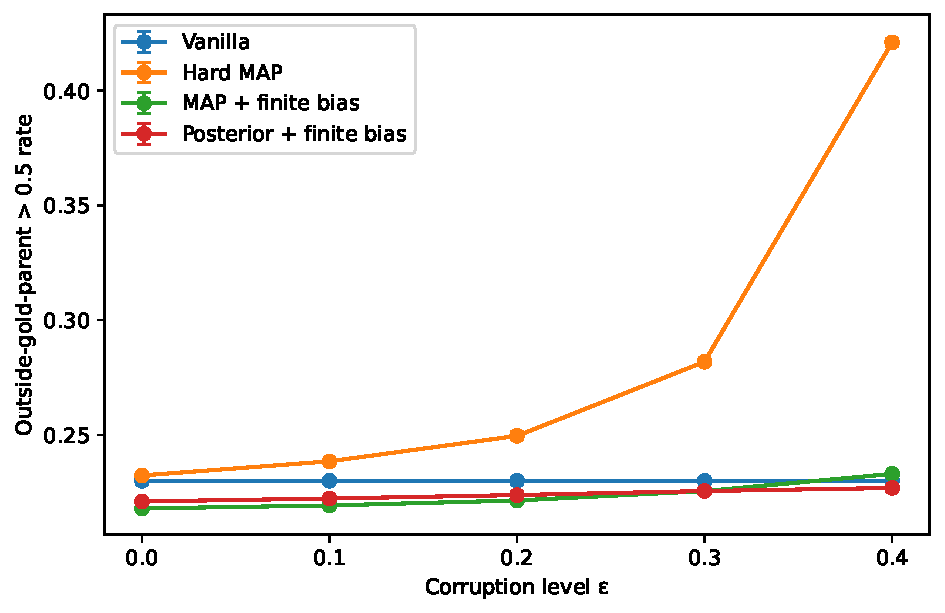
\includegraphics[width=\linewidth]{figures/fig_wos_corruption_catastrophic.pdf}
\smallskip
(b) Outside-gold-parent $>0.5$ rate
\end{minipage}
\caption{Controlled sensitivity analysis on the WOS predicted parent posterior. Error bars are 95\% $t$ intervals across ten paired head seeds.}
\label{fig:corruption}
\end{figure}

\section{Discussion}
\subsection{Robustness versus commitment}
Across controlled and external experiments, the stable result is a boundary condition on structural commitment rather than a universal ranking of mechanisms. When provenance is exact, hard gating is competitive in the synthetic assay and substantially better in WOS. Under predicted parents, finite-bias routing is markedly more robust than exact-support hard MAP. The matched WOS ablation sharpens the attribution: most of the gap survives after collapsing the parent posterior to MAP, so avoiding zero-support commitment is the dominant factor in this external assay. Document bootstrap intervals support the same interpretation: the MAP-finite-bias versus hard-MAP accuracy interval is well separated from zero, whereas the posterior-versus-MAP-finite-bias accuracy interval crosses zero.

Posterior preservation remains a distinct modeling choice. Under the matched finite-bias operator it lowers NLL, but in the unperturbed predicted condition it leaves more probability on alternative branches and increases several branch-concentration metrics. Under stronger corruption it becomes protective on accuracy, likelihood, and the outside-gold-parent threshold. This distinction is operationally relevant because knowledge-based systems may value calibrated uncertainty, branch concentration, or thresholded branch safety differently. Curated ontology membership or authoritative metadata can justify hard admissibility constraints; predicted taxonomy labels, entity-linking hypotheses, retrieval-source assignments, or learned branch projectors are qualitatively different.

\subsection{What ultrametric geometry contributes}
The strongest evidence for nested-shell geometry comes from the depth-four controlled assay: fixed ultrametric routing substantially exceeds ordinary tree distance and the fitted Poincar\'e baseline, while shuffled taxonomy collapses performance. The tuned prefix-ultrametric control slightly exceeds the fixed $\rho=0.2$ schedule, showing that this particular $p$-adic-compatible decay is not privileged within the same family. The WOS hierarchy is too shallow to discriminate among soft structural kernels after tuning and therefore neither confirms nor contradicts a multi-depth geometric advantage. A real deep hierarchy is required to test whether the synthetic longest-common-prefix advantage transfers externally.

The method should likewise not be advertised as a generic accuracy-improving hierarchical classifier. Under predicted WOS parents, no leaf-accuracy difference is detected between posterior ultrametric routing and vanilla classification. Its external value lies in avoiding brittle exact-support failures and in controlling how structural uncertainty is represented. In genuinely multi-depth structures, ultrametric shells provide an explicit shared-prefix ordering and differentiable soft-address extensions with analyzable sensitivity; in shallow taxonomies, simpler finite-bias branch-compatibility kernels may be sufficient.

\subsection{Architectural and semantic boundaries}
The synthetic validation and WOS transfer assay operate at different architectural locations by design. Only the synthetic experiment evaluates DSA inside attention; WOS applies compatibility after a frozen encoder. The matched MAP-plus-finite-bias control therefore decomposes posterior preservation from support hardness only at the post-encoder location. It does not establish that inserting DSA into ModernBERT's internal attention would improve a downstream task or that the same decomposition would hold end to end.

The WOS experiment also contains two uncertainty sources: the unperturbed parent posterior is induced by a supervised branch head on real text, whereas the subsequent $\varepsilon$-mixture is a controlled corruption intervention. The latter measures sensitivity rather than deployment prevalence. Finally, the synthetic wrong-vote intervention concerns provenance, not formal contradiction semantics: the model does not represent proposition-level $P/\neg P$ inconsistency. These boundaries define natural extensions rather than hidden claims.

\section{Limitations and Future Work}
Four limitations are most consequential. First, WOS-46985 has only one meaningful parent-to-leaf transition, so the distinctive multi-depth longest-common-prefix geometry remains externally untested; deeper independently defined ontologies are needed. Second, ModernBERT is frozen and routing is post-encoder, so end-to-end DSA and learned contextual passports remain future work. Third, the matched support-versus-posterior decomposition exists only for WOS; the synthetic attention-level uncertainty assay still couples MAP collapse with exact-support gating, and a distributional exact-support counterpart is not uniquely defined when a posterior supports several branches. Fourth, the multi-depth passport uses level-wise categorical marginals and therefore cannot encode arbitrary dependencies among complete paths.

The external evaluation is also deliberately narrow. The $\varepsilon$-mixture stress test is synthetic; confusion-derived perturbations, domain shift, retrieval-source uncertainty, and entity-linking errors would improve ecological validity. The WOS hierarchy requires a train-only modal repair of sparse label inconsistencies, all external results use one fixed split of one corpus, and the document bootstrap measures conditional test-document resampling rather than split-to-split or cross-dataset variability. Finally, the real-data assay shows no flat-accuracy advantage over a hierarchy-agnostic classifier. Applications concerned only with top-line classification accuracy may therefore receive little benefit from the present post-encoder operator.

\section{Conclusion}
This work studies the boundary between exact and uncertain hierarchical branch information when combining semantic evidence with structural knowledge. Hard constraints are effective when the relevant branch is known by construction. Under model-predicted branches, finite-bias routing is substantially more robust than exact-support hard MAP, and a matched WOS ablation shows that most of this external robustness gap is attributable to avoiding exact zeroing outside the MAP branch rather than to posterior preservation alone.

Differentiable prefix-ultrametric shells provide one controlled realization of this principle. They admit a true finite-depth zero diagonal, two hard-equivalent continuous extensions with provably different cross-depth sensitivity, a context-dependent leakage bound, and a direct attention-level DSA implementation. Controlled depth-four experiments show that nested-shell structure can matter strongly, while also showing that normalized hard gating is sufficient under exact provenance and that a tuned member of the same prefix-ultrametric family can slightly outperform the fixed $\rho=0.2$ schedule.

The evidence therefore supports a regime distinction rather than a universal policy. The exact-provenance assays function as a safety and equivalence check, not as an accuracy argument for soft routing: use hard hierarchical constraints when branch assignment is exact; use finite bias to avoid brittle zero-support failures when branch assignment is predicted; and treat full posterior preservation as a separate decision governing how uncertainty is distributed under that finite-bias operator. Ultrametric nested shells are especially relevant when a genuinely multi-depth hierarchy makes shared-prefix structure operationally meaningful.

\section*{CRediT authorship contribution statement}
\textbf{K. A. Ulizko:} Conceptualization, Methodology, Formal analysis, Software, Investigation, Data curation, Visualization, Writing -- original draft; \textbf{A. S. Vatian:} Conceptualization, Methodology, Supervision, Validation, Writing -- review \& editing, Project administration; \textbf{M. V. Ulizko:} Formal analysis, Validation, Writing -- review \& editing; \textbf{I. V. Tomilov:} Software, Validation, Data curation, Writing -- review \& editing; \textbf{N. F. Gusarova:} Conceptualization, Supervision, Validation, Writing -- review \& editing, Project administration.

\section*{Data and code availability}
Machine-readable controlled-experiment results and theorem-verification code and figure/table regeneration scripts are included with the reproducibility package supplied as supplementary material for peer review. The external experiment uses the public WOS-46985 corpus [40] and the open pretrained answerdotai/ModernBERT-base model [41]. The external pipeline records the exact model revision, embedding-extraction configuration, split definition, label-consistency audit, selected routing parameters, ten seed-level outputs, matched MAP-plus-finite-bias ablation, paired statistics, and document-bootstrap outputs required to reproduce the reported tables and corruption curves. No proprietary data are used. Upon acceptance, the authors will archive the complete reproducibility package in a persistent public repository and add its DOI or archival URL to the final manuscript.

\section*{Funding}
This work was supported by the Ministry of Science and Higher Education of the Russian Federation, Goszadanie (State Assignment) FSER-2025-0013.

\section*{Declaration of competing interest}
The authors declare that they have no known competing financial interests or personal relationships that could have appeared to influence the work reported in this paper.

\section*{Declaration of generative AI and AI-assisted technologies in the manuscript preparation process}
During the preparation of this work, the authors used ChatGPT (OpenAI) for manuscript organization, language revision, and consistency checks. After using this tool, the authors reviewed and edited the content as needed, independently verified the mathematical derivations, code, numerical outputs, and references, and take full responsibility for the content of the publication.

\section*{References}
\small
\begin{enumerate}[label={[\arabic*]},leftmargin=2.2em,itemsep=.28em,parsep=0pt]
\item P. Lewis, E. Perez, A. Piktus, et al., Retrieval-augmented generation for knowledge-intensive NLP tasks, in: Advances in Neural Information Processing Systems, 2020.
\item S. Pan, L. Luo, Y. Wang, C. Chen, J. Wang, X. Wu, Unifying large language models and knowledge graphs: A roadmap, IEEE Transactions on Knowledge and Data Engineering 36 (7) (2024) 3580--3599.
\item G. Agrawal, T. Kumarage, Z. Alghamdi, H. Liu, Can knowledge graphs reduce hallucinations in LLMs? a survey, in: Proceedings of NAACL, 2024, pp. 3947--3960.
\item S. Geng, M. Josifoski, M. Peyrard, R. West, Grammar-constrained decoding for structured NLP tasks without finetuning, in: Proceedings of EMNLP, 2023.
\item S. Ugare, R. Gumaste, T. Suresh, G. Singh, S. Misailovic, Flexible and efficient grammar-constrained decoding, arXiv:2502.05111 (2025).
\item P. Shaw, J. Uszkoreit, A. Vaswani, Self-attention with relative position representations, NAACL-HLT, 2018, pp. 464--468. doi:10.18653/v1/N18-2074.
\item C. Ying, T. Cai, S. Luo, S. Zheng, G. Ke, D. He, Y. Shen, T.-Y. Liu, Do transformers really perform badly for graph representation?, NeurIPS, 2021.
\item J. Zhu, J. Li, M. Zhu, L. Qian, M. Zhang, G. Zhou, Modeling graph structure in transformer for better AMR-to-text generation, EMNLP-IJCNLP, 2019, pp. 5459--5468. doi:10.18653/v1/D19-1548.
\item R. Ji, J. Ji, Transferring knowledge from structure-aware self-attention language model to sequence-to-sequence semantic parsing, COLING, 2022, pp. 3164--3174.
\item J. Qi, J. Tang, Z. He, X. Wan, Y. Cheng, C. Zhou, X. Wang, Q. Zhang, Z. Lin, RASAT: Integrating relational structures into pretrained seq2seq model for text-to-SQL, EMNLP, 2022, pp. 3215--3229. doi:10.18653/v1/2022.emnlp-main.211.
\item I. Beltagy, M. E. Peters, A. Cohan, Longformer: The long-document transformer, arXiv:2004.05150 (2020).
\item M. Zaheer, G. Guruganesh, A. Dubey, et al., Big Bird: Transformers for longer sequences, NeurIPS, 2020.
\item J. Chen, C. Li, Y. Yuan, A. C. Yao, Hierarchical attention generates better proofs, ACL, 2025, pp. 17506--17520. doi:10.18653/v1/2025.acl-long.856.
\item X. L. Dong, E. Gabrilovich, G. Heitz, W. Horn, N. Lao, K. Murphy, T. Strohmann, S. Sun, W. Zhang, Knowledge Vault: A web-scale approach to probabilistic knowledge fusion, KDD, 2014, pp. 601--610. doi:10.1145/2623330.2623623.
\item X. Chen, M. Chen, W. Shi, Y. Sun, C. Zaniolo, Embedding uncertain knowledge graphs, AAAI 33 (2019) 3363--3370. doi:10.1609/aaai.v33i01.33013363.
\item S. H. Bach, M. Broecheler, B. Huang, L. Getoor, Hinge-loss Markov random fields and probabilistic soft logic, JMLR 18 (109) (2017) 1--67.
\item W. Shen, J. Wang, J. Han, Entity linking with a knowledge base: Issues, techniques, and solutions, IEEE TKDE 27 (2) (2015) 443--460. doi:10.1109/TKDE.2014.2327028.
\item M. Nickel, D. Kiela, Poincar\'e embeddings for learning hierarchical representations, NeurIPS, 2017.
\item M. Nickel, D. Kiela, Learning continuous hierarchies in the Lorentz model of hyperbolic geometry, ICML, 2018, pp. 3779--3788.
\item O.-E. Ganea, G. B\'ecigneul, T. Hofmann, Hyperbolic neural networks, NeurIPS, 2018.
\item I. Chami, R. Ying, C. R\'e, J. Leskovec, Hyperbolic graph convolutional neural networks, NeurIPS, 2019.
\item C. Gulcehre, M. Denil, M. Malinowski, et al., Hyperbolic attention networks, ICLR, 2019.
\item Q. Liu, M. Nickel, D. Kiela, Graph transformer networks with hyperbolic geometry, arXiv:2106.07350 (2021).
\item M. Yang, H. Verma, D. C. Zhang, J. Liu, I. King, R. Ying, Hypformer: Exploring efficient hyperbolic transformer fully in hyperbolic space, arXiv:2407.01290 (2024).
\item F. Murtagh, G. Downs, P. Contreras, Hierarchical clustering of massive, high dimensional data sets by exploiting ultrametric embedding, SIAM J. Sci. Comput. 30 (2008) 707--730. doi:10.1137/060676532.
\item E. W. Holman, The relation between hierarchical and euclidean models for psychological distances, Psychometrika 37 (4) (1972) 417--423. doi:10.1007/BF02291218.
\item C.-M. Cuadras, F. Carmona, Dimensionalitat euclidiana de les distancies ultram\`etriques, Q\"uestii\'o 7 (1) (1983) 353--358.
\item T. Faver, K. Kochalski, M. K. Murugan, H. Verheggen, E. Wesson, A. Weston, Roundness properties of ultrametric spaces, Glasgow Mathematical Journal 56 (3) (2014) 519--535. doi:10.1017/S0017089513000438.
\item A. F. T. Martins, Learning with the $p$-adics, arXiv:2512.22692 (2025).
\item G. L. R. N'guessan, v-PuNNs: van der Put neural networks for transparent ultrametric representation learning, arXiv:2508.01010 (2025).
\item B. Toni, Beyond Archimedean intelligence: Toward an intrinsic $p$-adic theory of learning, arXiv:2607.14562 (2026).
\item W. A. Z\'u\~niga-Galindo, Deep neural networks: A formulation via non-Archimedean analysis, Journal of Fourier Analysis and Applications 32 (2026) 77. doi:10.1007/s00041-026-10290-y.
\item S. Bae, D. Lee, Numbers already carry their own embeddings, arXiv:2606.14108 (2026).
\item R. B. Quni-Gudzinas, A proof-of-concept for auditable attention using ultrametric tree distances, Tech. rep., Zenodo (2026). doi:10.5281/zenodo.19648274.
\item E. Jang, S. Gu, B. Poole, Categorical reparameterization with Gumbel-softmax, ICLR, 2017.
\item C. J. Maddison, A. Mnih, Y. W. Teh, The Concrete distribution: A continuous relaxation of discrete random variables, ICLR, 2017.
\item A. F. T. Martins, R. F. Astudillo, From softmax to sparsemax: A sparse model of attention and multi-label classification, ICML, 2016, pp. 1614--1623.
\item B. Peters, V. Niculae, A. F. T. Martins, Sparse sequence-to-sequence models, ACL, 2019, pp. 1504--1519.
\item K. Kowsari, D. E. Brown, M. Heidarysafa, K. Jafari Meimandi, M. S. Gerber, L. E. Barnes, HDLTex: Hierarchical deep learning for text classification, ICMLA, 2017, pp. 364--371. doi:10.1109/ICMLA.2017.0-134.
\item K. Kowsari, D. Brown, M. Heidarysafa, K. Jafari Meimandi, M. Gerber, L. Barnes, Web of Science, Mendeley Data, Version 5 (2018). doi:10.17632/9rw3vkcfy4.5.
\item B. Warner, A. Chaffin, B. Clavi\'e, O. Weller, O. Hallstr\"om, S. Taghadouini, A. Gallagher, R. Biswas, F. Ladhak, T. Aarsen, N. Cooper, G. Adams, J. Howard, I. Poli, Smarter, better, faster, longer: A modern bidirectional encoder for fast, memory efficient, and long context finetuning and inference, arXiv:2412.13663 (2024).
\end{enumerate}

\end{document}
